%%%%%%%%%%%%%%%%%%%%%%%%%%%%%%%%%%%%%%%%%
% Beamer Presentation
% LaTeX Template
% Version 1.0 (10/11/12)
%
% This template has been downloaded from:
% http://www.LaTeXTemplates.com
%
% License:
% CC BY-NC-SA 3.0 (http://creativecommons.org/licenses/by-nc-sa/3.0/)
%
%%%%%%%%%%%%%%%%%%%%%%%%%%%%%%%%%%%%%%%%%

%----------------------------------------------------------------------------------------
%	PACKAGES AND THEMES
%----------------------------------------------------------------------------------------

\documentclass[UTF8,aspectratio=169,14pt]{ctexbeamer}

\usepackage{hyperref}
\hypersetup{
	colorlinks=true,
	linkcolor=red,
	anchorcolor=blue,
	citecolor=green
}

\mode<presentation> {
	
	% The Beamer class comes with a number of default slide themes
	% which change the colors and layouts of slides. Below this is a list
	% of all the themes, uncomment each in turn to see what they look like.
	
	%\usetheme{default}
	%\usetheme{AnnArbor}
	%\usetheme{Antibes}
	%\usetheme{Bergen}
	%\usetheme{Berkeley}
	%\usetheme{Berlin}
	%\usetheme{Boadilla}
	%\usetheme{CambridgeUS}
	%\usetheme{Copenhagen}
	%\usetheme{Darmstadt}
	%\usetheme{Dresden}
	%\usetheme{Frankfurt}
	%\usetheme{Goettingen}
	%\usetheme{Hannover}
	%\usetheme{Ilmenau}
	%\usetheme{JuanLesPins}
	%\usetheme{Luebeck}
	\usetheme{Madrid}
	%\usetheme{Malmoe}
	%\usetheme{Marburg}
	%\usetheme{Montpellier}
	%\usetheme{PaloAlto}
	%\usetheme{Pittsburgh}
	%\usetheme{Rochester}
	%\usetheme{Singapore}
	%\usetheme{Szeged}
	%\usetheme{Warsaw}
	
	% As well as themes, the Beamer class has a number of color themes
	% for any slide theme. Uncomment each of these in turn to see how it
	% changes the colors of your current slide theme.
	
	%\usecolortheme{albatross}
	%\usecolortheme{beaver}
	%\usecolortheme{beetle}
	%\usecolortheme{crane}
	%\usecolortheme{dolphin}
	%\usecolortheme{dove}
	%\usecolortheme{fly}
	%\usecolortheme{lily}
	%\usecolortheme{orchid}
	%\usecolortheme{rose}
	%\usecolortheme{seagull}
	%\usecolortheme{seahorse}
	%\usecolortheme{whale}
	%\usecolortheme{wolverine}
	
	%\setbeamertemplate{footline} % To remove the footer line in all slides uncomment this line
	%\setbeamertemplate{footline}[page number] % To replace the footer line in all slides with a simple slide count uncomment this line
	
	%\setbeamertemplate{navigation symbols}{} % To remove the navigation symbols from the bottom of all slides uncomment this line
}

\usepackage{graphicx} % Allows including images
\graphicspath{{./figs/}}
\usepackage{booktabs} % Allows the use of \toprule, \midrule and \bottomrule in tables
\usepackage{longtable}
\usepackage{listings}
\usepackage{xcolor}
\lstset{numbers=left, %设置行号位置
	numberstyle=\tiny, %设置行号大小
	keywordstyle=\color{blue}, %设置关键字颜色
	commentstyle=\color[cmyk]{1,0,1,0}, %设置注释颜色
	frame=single, %设置边框格式
	escapeinside=``, %逃逸字符(1左面的键),用于显示中文
	%breaklines, %自动折行
	extendedchars=false, %解决代码跨页时,章节标题,页眉等汉字不显示的问题
	xleftmargin=2em,xrightmargin=2em, aboveskip=1em, %设置边距
	tabsize=4, %设置tab空格数
	showspaces=false %不显示空格
}
% Fonts
% \usepackage{libertine}
% \setmonofont{Courier}
\setCJKsansfont[ItalicFont=Noto Serif CJK SC Black, BoldFont=Noto Sans CJK SC Black]{Noto Sans CJK SC}

%\def\imagepath{./resources/graphics}
%\usepackage[imagepath=\imagepath]{ditaa}
%\graphicspath{ {\imagepath/} }


%\usepackage{pgfpages}
%\setbeameroption{show notes on second screen}
%%----------------------------------------------------------------------------------------
%	TITLE PAGE
%----------------------------------------------------------------------------------------

\title[第9讲]{第九讲 :进程和线程} % The short title appears at the bottom of every slide, the full title is only on the title page
\subtitle{第9节:进程地址空间与熔断(meltdown)漏洞}
\author{向勇、陈渝} % Your name
\institute[清华大学] % Your institution as it will appear on the bottom of every slide, may be shorthand to save space
{
	清华大学计算机系 \\ % Your institution for the title page
	\medskip
	\textit{xyong,yuchen@tsinghua.edu.cn} % Your email address
}
\date{\today} % Date, can be changed to a custom date


\begin{document}

\begin{frame}
\titlepage % Print the title page as the first slide
\end{frame}

%----------------------------------------------
\begin{frame}
\frametitle{提纲} % Table of contents slide, comment this block out to remove it
\tableofcontents % Throughout your presentation, if you choose to use \section{} and \subsection{} commands, these will automatically be printed on this slide as an overview of your presentation
\end{frame}
%----------------------------------------------
%%	PRESENTATION SLIDES
%----------------------------------------------
%------------------------------------------------
\section{第9节:进程地址空间与熔断(meltdown)漏洞}% Sections can be created in order to organize your presentation into discrete blocks, all sections and subsections are automatically printed in the table of contents as an overview of the talk
%------------------------------------------------
\subsection{背景知识回顾} % A subsection can be created just before a set of slides with a common theme to further break down your presentation into chunks
%------------------------------------------------
\begin{frame}[fragile]
    \frametitle{侧信道攻击}
    \begin{block}{}
    假设有abc三个变量,其中a没有访问权限,但是b和c可以访问,此时执行下面这个条件表达式:
    \begin{lstlisting}[language = C]
        x = a ?b:c
    \end{lstlisting}
    \end{block} \pause
	    \begin{itemize}
	        \item a无法访问,系统会直接报错! \pause
	        \item 采用多流水线的CPU在检查a的访问权限时,继续往下执行。 \pause
	        \item a的权限检查完成时,CPU已依据a的值完成了b或者c的读取,只是还没有赋值给x。
	    \end{itemize}
\end{frame}
%------------------------------------------------
\begin{frame}[fragile]
    \frametitle{侧信道攻击的影响}
	    \begin{itemize}
	        \item 虽然表达式报错,但再次访问变量的速度会变快;
	        \item 后续访问b和c时,依据访问时间长短,可猜到a的值; \pause
	        \item 这个问题导致了2018年元旦前后熔断漏洞(CVE-2017-5754: meltdown); \pause
	        \item 需要操作系统来补救这个CPU设计问题:KAISER \pause
	        \item 类似问题不止这一个......
	    \end{itemize}
\end{frame}
%------------------------------------------------

% #### 背景
% 
% 假设有abc三个地址,其中a地址没有访问的权限,但是b和c可以访问,此时执行下面这个条件表达式:
% 
% x= a?b:c
% 
% 表面看来,由于a地址无法访问,所以系统会直接报错!
% 但实际上,CPU为了加快执行速度,会采用多流水线作业方式。它会在检查a是否可访问的同时,预先就往下执行了。
% 等到权限检查结果回来,已经根据a的结果完成了b或者c的加载,只是还没有赋给x而已。经过加载的b或者c会在缓存里。虽然报错了,但如果再次访问就会比较快。
% 于是再次访问b和c,根据返回的时间快慢,就可以猜到a的内容!
% 
%------------------------------------------------
\begin{frame}
    \frametitle{CPU高速缓存结构(Intel Skylake)}
	  %% figure
	  	\begin{figure}
	  	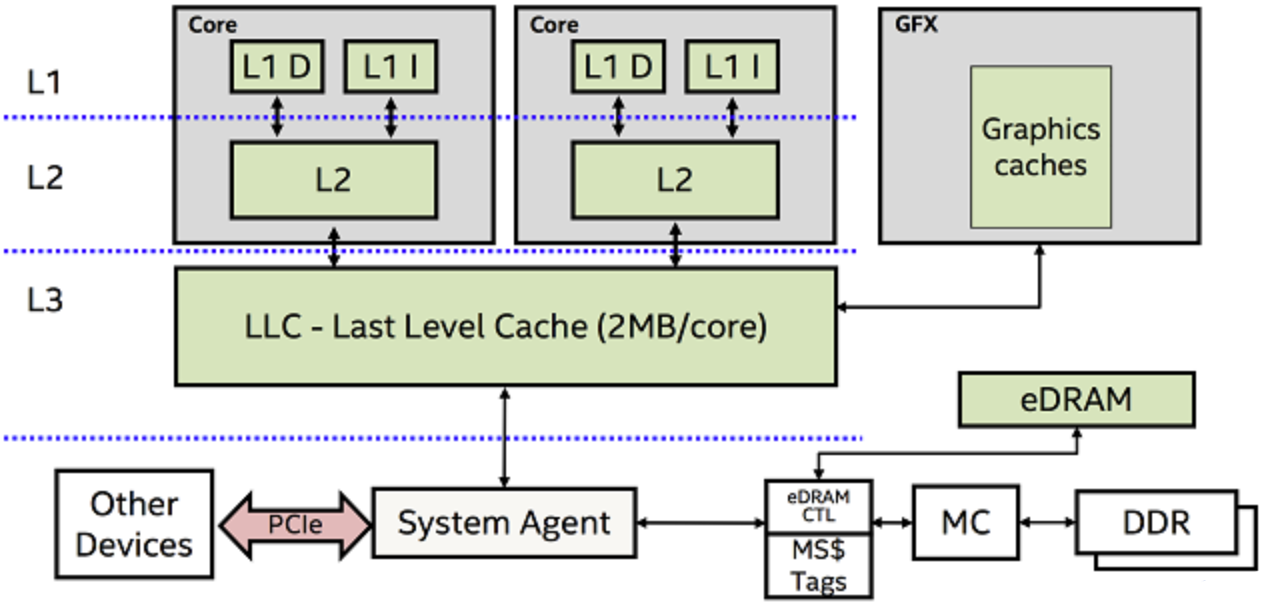
\includegraphics[width=0.9\linewidth]{figs/cache-in-skylake.png}
	%  	\caption{xxxx}
	  	\end{figure}
\end{frame}
%------------------------------------------------
\begin{frame}
    \frametitle{各级存储结构的访问延迟}
\begin{table}[]
\begin{tabular}{|l|l|}
\cline{1-2}
访问类型        & 延迟        \\ \cline{1-2} 
L1 cache命中  & 约4个时钟周期  \\ \cline{1-2}
L2 cache 命中 & 约10个时钟周期 \\ \cline{1-2}
L3 cache命中  & 约40个时钟周期 \\ \cline{1-2}
访问本地DDR & 约60 纳秒 \\ \cline{1-2}
访问远端内存节点DDR & 约100 纳秒  \\ \cline{1-2}
\end{tabular}
\end{table}

\end{frame}
%------------------------------------------------
% #### CPU高速缓存结构(Intel Skylake)
% 
% [How Does CPU Cache Work?](https://www.makeuseof.com/tag/what-is-cpu-cache/)
% 
% ![cache-in-skylake](figs/cache-in-skylake.png)
% 
% https://mp.weixin.qq.com/s/zlspXeDGlAEzVsq2h6gg8w
% 
% 各级存储结构的访问延迟
% 
% | 访问类型            | 延迟           |
% | ------------------- | -------------- |
% | L1 cache命中        | 约4个时钟周期  |
% | L2 cache 命中       | 约10个时钟周期 |
% | L3 cache命中        | 约40个时钟周期 |
% | 访问本地DDR         | 约60 纳秒      |
% | 访问远端内存节点DDR | 约100纳秒      |
% 
%------------------------------------------------
\begin{frame}
  %% columns
      \begin{columns}
      \begin{column}{0.4\textwidth}
	    \frametitle{指令执行的乱序优化(Intel Skylake)}
		  %% figure
		  	\begin{figure}
		  	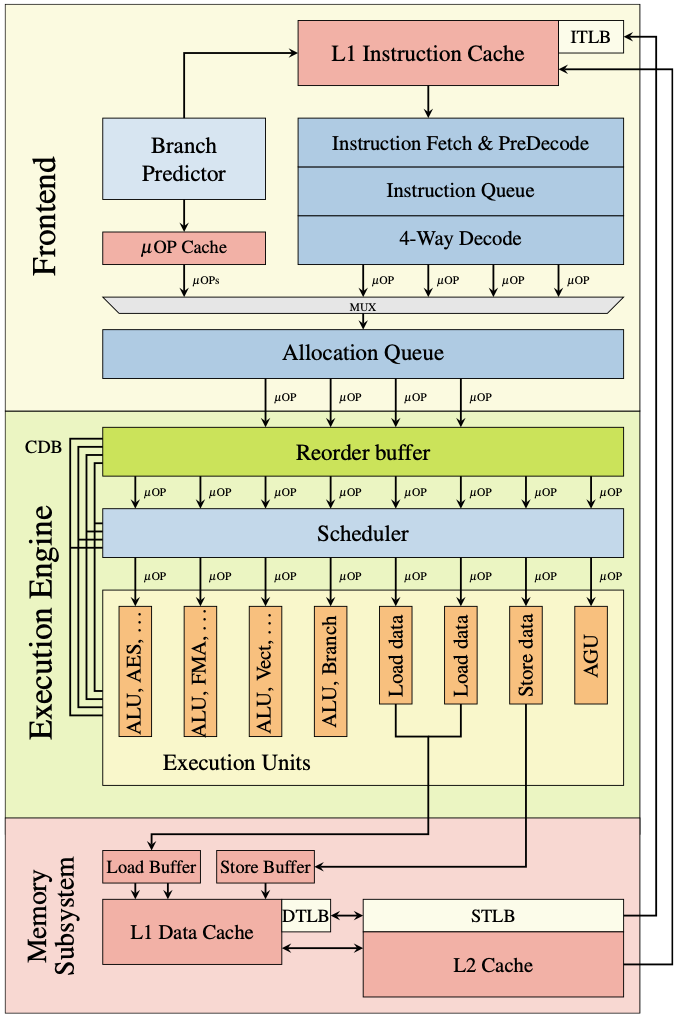
\includegraphics[width=0.75\linewidth]{figs/skylake-out-of-order.png}
		%  	\caption{xxxx}
		  	\end{figure}
      \end{column} \pause
      \begin{column}{0.6\textwidth}
		   \begin{block}{乱序执行过程}
		    \begin{itemize}
		        \item 获取指令和解码:保放到执行缓冲区 \pause
		        \item 乱序执行指令:保存在结果序列中 \pause
		        \item 退休期Retired Circle:重新排列结果序列及安全检查(如地址访问的权限检查),提交结果到寄存器
		    \end{itemize}
		    \end{block}
      \end{column}
      \end{columns}
\end{frame}
%------------------------------------------------
% #### 指令执行的乱序优化(Intel Skylake)
% https://meltdownattack.com/meltdown.pdf
% Meltdown: Reading Kernel Memory from User Space
% Figure 1: Simplified illustration of a single core of the Intel’s Skylake microarchitecture
% 
% ![skylake-out-of-order](figs/skylake-out-of-order.png)
% 
% https://www.zhihu.com/question/265012502?utm_medium=social&utm_source=wechat_session&from=groupmessage&isappinstalled=0
% 
% 乱序执行可以简单的分为三个阶段
% 
% 1. 获取指令,解码后存放到执行缓冲区Reservations Stations
% 2. 乱序执行指令,结果保存在一个结果序列中
% 3. 退休期Retired Circle,重新排列结果序列及安全检查(如地址访问的权限检查),提交结果到寄存器
% 
%------------------------------------------------
\begin{frame}
    \frametitle{CPU异常指令执行}
  %% figure
  	\begin{figure}
  	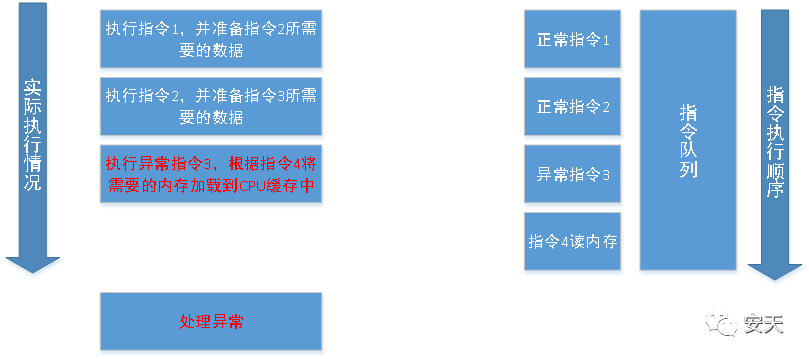
\includegraphics[width=0.9\linewidth]{figs/exception.png}
%  	\caption{xxxx}
  	\end{figure}

\end{frame}
%------------------------------------------------
% #### CPU异常指令执行
% 
% https://www.freebuf.com/vuls/159269.html
% CPU异常指令执行
% 
% ![exception](figs/exception.png)
% 
%------------------------------------------------
\begin{frame}
    \frametitle{CPU数据访问权限和地址合法性检查}
  %% figure
  	\begin{figure}
  	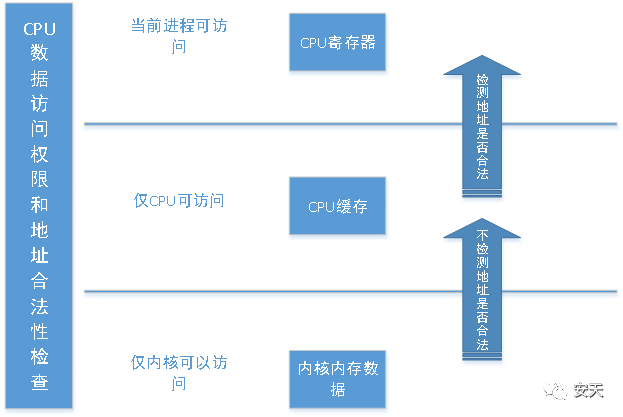
\includegraphics[width=0.65\linewidth]{figs/right-check.png}
%  	\caption{xxxx}
  	\end{figure}

\end{frame}
%------------------------------------------------
% #### CPU数据访问权限和地址合法性检查
% 
% https://www.freebuf.com/vuls/159269.html
% 图3 CPU数据访问权限和地址合法性检查
% 
% ![right-check](figs/right-check.png)
% 
%------------------------------------------------
\subsection{熔断漏洞} % A subsection can be created just before a set of slides with a common theme to further break down your presentation into chunks
%------------------------------------------------
\begin{frame}
    \frametitle{熔断漏洞(CVE-2017-5754):核心攻击代码}
	  %% figure
	  	\begin{figure}
	  	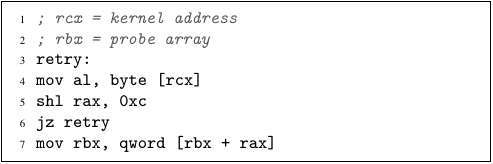
\includegraphics[width=0.6\linewidth]{figs/meltdown-poc.jpg}
%	  	\caption{xxxx}
	  	\end{figure} \pause
		    \begin{itemize}
		        \item 假定已分配一块$2^{8}=256$个4KB页面大小的内存区域($256*4096$)作为探测数组(probe array),并保证该内存块未被缓存;要非法访问的内存地址在rcx; \pause
		        \item 通过mov指令读取一个字节到rax;该指令会产生异常,但在异常产生前,CPU已部分完成读取操作; \pause
		        \item 假定读到的值是$i$,则CPU会继续访问探测数组的第$i*4096$个元素,导致CPU缓存该元素; \pause
		        \item 测量所有256个页面内存的访问时间,就可估计出$i$的值。
		    \end{itemize}
\end{frame}
%------------------------------------------------
% #### 熔断漏洞(CVE-2017-5754):利用过程
% 
% https://meltdownattack.com/meltdown.pdf
% Meltdown: Reading Kernel Memory from User Space
% 
% ![meltdown-poc](figs/meltdown-poc.jpg)
% 
%  1. 接收者开辟一段2^8=256个page大小的内存(256*4096)作为probe array,并保证这部分内存未被缓存。
%  2. 假设要访问的非法内存的地址存在rcx, % 通过mov指令读取位于rcx地址的内存中的一个字节,存在rax中,这条指令将来会产生异常,然而在异常产生前,就可以通过transient % instructions把读取的内容发送出去:
%  3. 假设读取的值是i,那么就在transient instructions里面访问probe array的第i*4096个元素,这会导致第i*4096个元素被缓存。
%  4. 接收者通过测量所有的256个page的内存的访问时间,就可以知道i的值了。
% 
%------------------------------------------------
\begin{frame}
    \frametitle{熔断漏洞:攻击过程示意图}
  %% figure
  	\begin{figure}
  	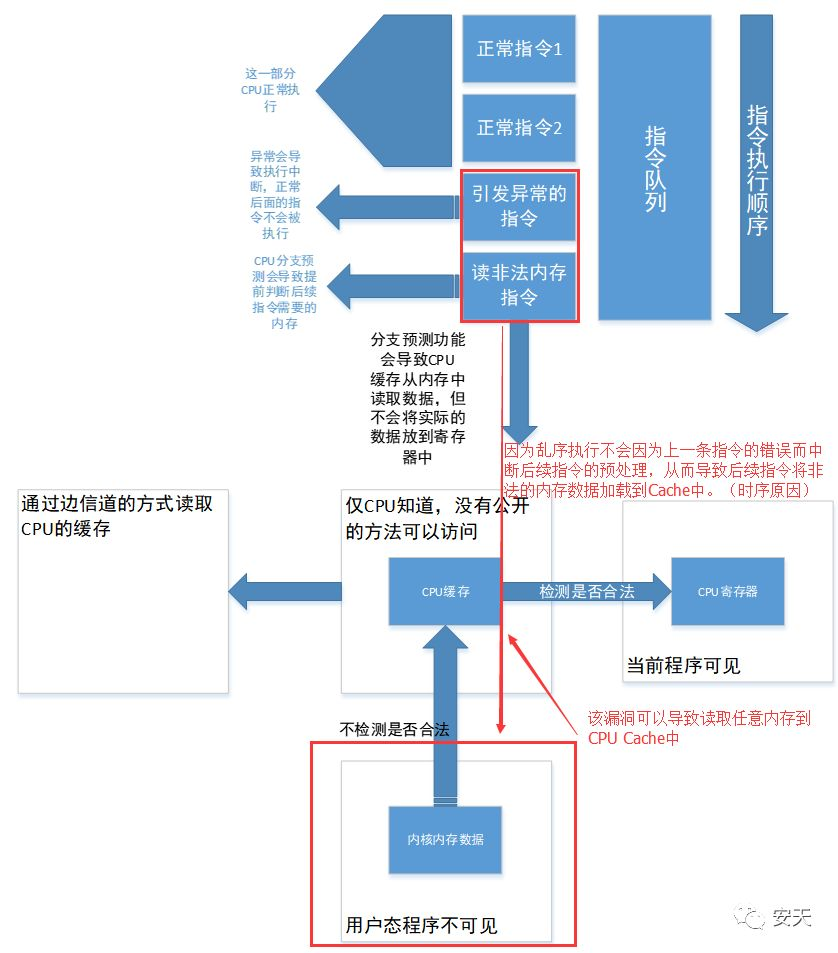
\includegraphics[width=0.4\linewidth]{figs/meltdown-method.jpg}
  	\caption{xxxx}
  	\end{figure}

\end{frame}
%------------------------------------------------
% #### 熔断漏洞:原理
% https://mp.weixin.qq.com/s/2FvvFUT8taRPv6GOHzNW-g
% 图4 漏洞原理图
% 
% ![meltdown-method](figs/meltdown-method.jpg)
% 
%------------------------------------------------
\begin{frame}
    \frametitle{熔断漏洞:在用户态读取内核数据}
  %% figure
  	\begin{figure}
  	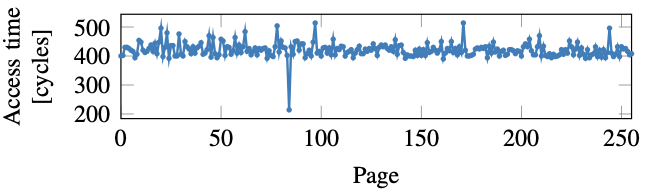
\includegraphics[width=1.0\linewidth]{figs/access-duration.png}
%  	\caption{xxxx}
  	\end{figure}

\end{frame}
%------------------------------------------------
% #### 熔断漏洞:在用户态读取内核数据
% 
% https://meltdownattack.com/meltdown.pdf
% Meltdown: Reading Kernel Memory from User Space
% Figure 4
% 
% ![access-duration](figs/access-duration.png)
% 
%------------------------------------------------
\subsection{进程用户态和内核态的隔离} % A subsection can be created just before a set of slides with a common theme to further break down your presentation into chunks
%------------------------------------------------
\begin{frame}
    \frametitle{KPTI: Kernel page-table isolation}
	  %% figure
	  	\begin{figure}
	  	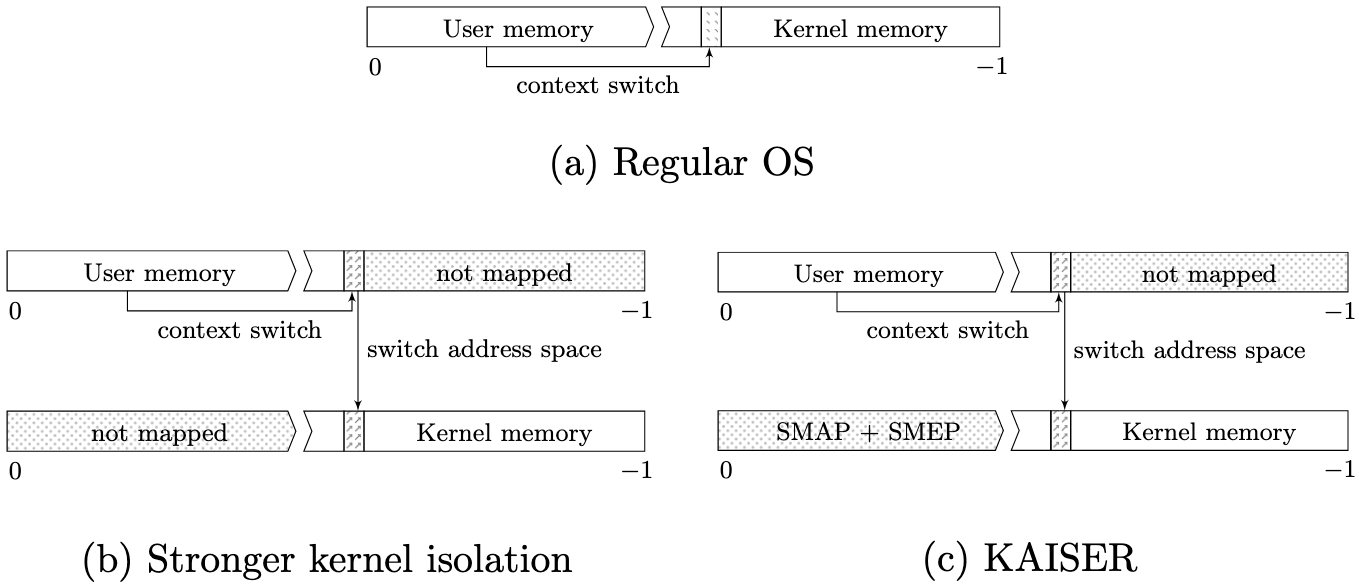
\includegraphics[width=0.8\linewidth]{figs/kaiser.png}
%	  	\caption{xxxx}
	  	\end{figure} \pause

        (a) Kernel is mapped into the address space \pause

        (b) Stronger kernel isolation: only  interrupt  handling  code  is mapped \pause
        
        (c) KAISER: prevent invalid references (SMAP) and prevent execution (SMEP)
\end{frame}
%------------------------------------------------
% #### KPTI: Kernel page-table isolation
% https://gruss.cc/files/kaiser.pdf
% KASLR is Dead: Long Live KASLR
% Fig. 2
% 
% ![kaiser](figs/kaiser.png)
% 
% (a) The kernel is mapped into the address space of every user process.
% (b) Theoretical concept of stronger kernel isolation. It splits the address spacesand  only  interrupt  handling  code  is  % mapped  in  both  address  spaces. 
% (c)  Forcompatibility with x86 Linux, KAISER relies on SMAP to prevent invalid usermemory references and SMEP to prevent % execution of user code in kernel mode.
% 
% supervisor-mode access prevention (SMAP) and supervisor-mode execution prevention (SMEP)
% 
%------------------------------------------------
\begin{frame}
    \frametitle{Shadow address space in KAISER}
	  %% figure
	  	\begin{figure}
	  	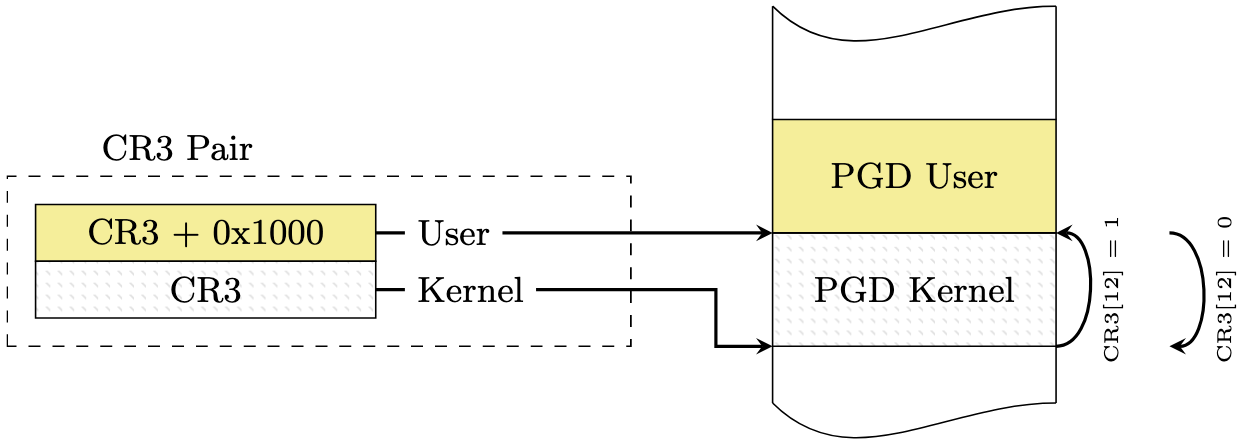
\includegraphics[width=0.8\linewidth]{figs/kaiser-shadow-AS.png}
%	  	\caption{xxxx}
	  	\end{figure}
    \begin{itemize}
        \item KAISER: Kernel Address Isolation to have Side channels Efficiently Removed \pause
        \item PML4 of user address space and kernel addressspace are placed next to each other in physical memory.
    \end{itemize}

\end{frame}
%------------------------------------------------
% #### Shadow address space in KAISER
% https://gruss.cc/files/kaiser.pdf
% KASLR is Dead: Long Live KASLR
% Fig. 3: Shadow address space
% 
% Kernel Address Isolation to have Side channels Efficiently Removed, KAISER
% 
% ![kaiser-shadow-AS](figs/kaiser-shadow-AS.png)
% 
% PML4 of user address space and kernel addressspace are placed next to each other in physical memory.
% 
% https://en.wikipedia.org/wiki/Kernel_page-table_isolation
% 
% 
%------------------------------------------------
\begin{frame}
    \frametitle{“骑士” 漏洞(CVE-2019-11157)}
    \begin{itemize}
        \item 动态电源管理模块DVFS(Dynamic Voltage and Frequency Scaling)允许多核处理器根据负载信息采用相应的频率和电压运行,以降低处理器的功耗。 \pause
        \item 当一个核出现电压和频率不太匹配(如电压偏低无法满足较高频率运行需求)时,系统就会出现短暂“故障”。 \pause
        \item 故障对系统行为结果的干扰会泄露出的系统行为信息。 \pause
    \end{itemize}
  %% figure
  	\begin{figure}
  	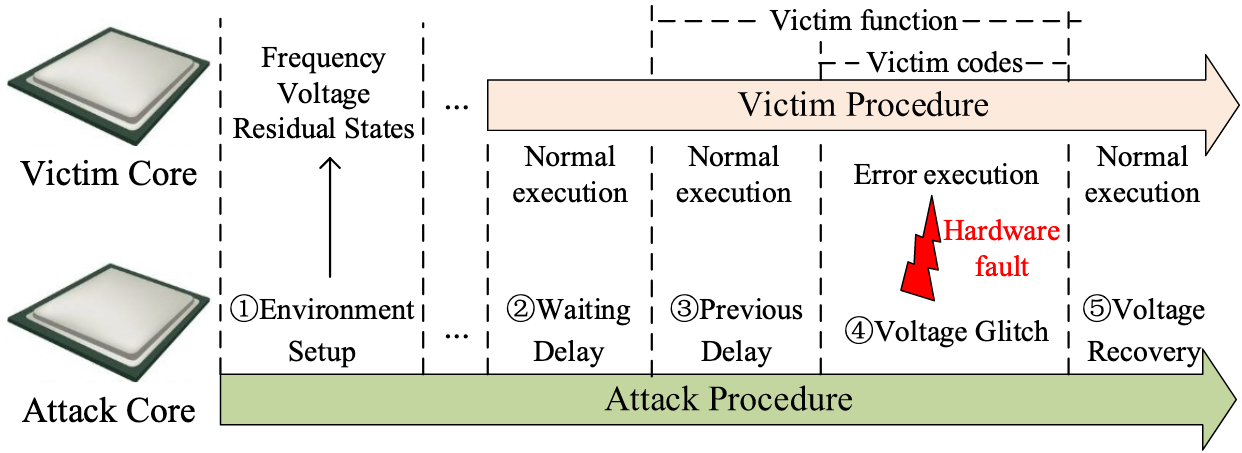
\includegraphics[width=0.8\linewidth]{figs/VoltJockey.png}
%  	\caption{xxxx}
  	\end{figure}

\end{frame}
%------------------------------------------------
% #### “骑士” 漏洞(CVE-2019-11157)
% 
% http://voltjockey.com/flies/paper/2.pdf
% VoltJockey: Breaking SGX by Software-ControlledVoltage-Induced Hardware Faults
% Fig. 1.   Overview of our voltage-induced fault attack
% 
% ![VoltJockey](figs/VoltJockey.png)
% 
% 动态电源管理模块DVFS(Dynamic Voltage and Frequency Scaling)允许多核处理器根据负载信息采用相应的频率和电压运行,以降低处理器的功耗。
% 当一个核出现电压和频率不太匹配(如电压偏低无法满足较高频率运行需求)时,系统就会出现短暂“故障”。
% 故障对系统行为结果的干扰会泄露出的系统行为信息。
%----------------------------------------------

\end{document}
